%%%%%%%%%%%%%%%%%%%%%%%%%%%%%%%%%%%%
% This is the template for submission to ISCA 2018
% The cls file is a modified from  'sig-alternate.cls'
%%%%%%%%%%%%%%%%%%%%%%%%%%%%%%%%%%%%

\documentclass{sig-alternate}
\usepackage{mathptmx} % This is Times font

\newcommand{\ignore}[1]{}
\usepackage{fancyhdr}
\usepackage[normalem]{ulem}
\usepackage[hyphens]{url}
\usepackage{microtype}

% Always include hyperref last
\usepackage[bookmarks=true,breaklinks=true,letterpaper=true,colorlinks,linkcolor=black,citecolor=blue,urlcolor=black]{hyperref}

% Ensure letter paper
\pdfpagewidth=8.5in
\pdfpageheight=11in


%%%%%%%%%%%---SETME-----%%%%%%%%%%%%%
\newcommand{\iscasubmissionnumber}{NaN}
%%%%%%%%%%%%%%%%%%%%%%%%%%%%%%%%%%%%

\fancypagestyle{firstpage}{
  \fancyhf{}
\renewcommand{\headrulewidth}{0pt}
  \fancyhead[C]{\normalsize{ISCA 2018 Submission
      \textbf{\#\iscasubmissionnumber} \\ Confidential Draft: DO NOT DISTRIBUTE}}
  \fancyfoot[C]{\thepage}
}

\pagenumbering{arabic}

%%%%%%%%%%%---SETME-----%%%%%%%%%%%%%
\title{In Class Branch Prediction Competition}
\author{Arham Chopra, 14130 \\ Ayush Tulsyan, 14167}
%%%%%%%%%%%%%%%%%%%%%%%%%%%%%%%%%%%%

\begin{document}
\maketitle
\thispagestyle{firstpage}
\pagestyle{plain}

\begin{abstract}

In this report we present a comparison of the 3 famous branch predictors namely gshare, bimode, and agree in terms of the MPPKI on the provided traces. After that we present a new branch predictor that is based on the combination of bimode and agree predictors. Then we give a detailed description of the hardware budget of our predictor.

\end{abstract}

\section{Background Information}

The results obtained on running our implementations of bimode and agree predictors are as follows (corresponding results obtained for gshare have also been added for comparision). The simulation were done by using traces from CBP framework. The hardware budget was kept uniform across these predictors which was 64 Kilobits.

\begin{table}[h]

\caption{Agree\cite{agreepaper}, Bimode\cite{bimodepaper} and Gshare\cite{gsharepaper}}
\centering

\begin{tabular}{llll}

\hline
Trace & Agree & Bimode & Gshare \\
\hline
DIST-INT-1 & 8.265 & 8.023 & 7.907 \\
DIST-INT-2 & 9.206 & 8.844 & 8.708 \\
DIST-INT-3 & 13.184 & 13.854 & 13.357 \\
DIST-MM-1 & 9.164 & 9.230 & 9.119 \\
DIST-MM-2 & 10.730 & 10.884 & 10.854 \\
DIST-SERV-1 & 5.319 & 3.660 & 5.691 \\
DIST-SERV-2 & 5.031 & 3.711 & 5.897 \\
DIST-SERV-3 & 5.999 & 5.698 & 7.235 \\
DIST-SERV-4 & 6.574 & 4.720 & 7.009 \\
DIST-SERV-5 & 5.431 & 4.541 & 6.767 \\
\hline

\end{tabular}

\end{table}

As can be observed, the gshare predictor performs better in the INT and MM traces. It is however beaten in the SERV traces and by a relatively large margin. It is also observed that bimode and agree perform better than gshare on different traces. More precisely, they express some sor of complementary behavior, which is one of the reasons for our combined predictor.\par

\section{Motivation}
One of the motivations for our combined predictor as already mentioned in the previous section is that both agree and bimode perform well as compared to gshare on different sets of traces. Thus if these can be combined in some fashion, the resultant predictor would be able to beat gshare on most of the traces. This is not so straight forward in any case. Since, the two predictors, Agree and bi-mode, were able to beat Gshare when they had the complete 64 Kb budget allocated to themselves. When we are implementing a hybrid predictor with a fixed budget, the two predictors will share the budget and will perform worse individually. \par

The other motivation for combining them is negative interference(aliasing). Both of the predictors attempt to reduce the problem of negative interference. By combining them we might be able to reduce this problem to a larger extent as possible by both separately.

\section{Description Joint-Agree-Bimode}

The PHT, consisting of 2 bit saturating counters, is divided into two equal parts like the bimode predictor, these two parts correspond to the two different behaviours of the branches. During a prediction the global history register(GHR) is xored with the branch address and then masked with the size of the PHTs to obtain the index to the 2-bit counters. 2 bit counters from each PHT are taken. A choice predictor, table of 2 bit saturating counters similar to the bimode predictor, is used to determine which of the two counters should be chosen for the final prediction.

The difference and where agree comes into the picture is how the prediction is done after the appropriate 2 bit counter is chosen. A bias bit is stored for each branch, like the agree predictor, and the prediction made by the 2 bit counter is matched with the bias bit to make the final decision regarding the branch outcome. Similar to the agree predictor, if the bias bit matches with the MSB of the 2 bit counter then  the predicted outcome is taken and it is not taken in case they do not match.

The update criteria of the combined predictor is also quite similar to the individual components. The 2 bit saturating counter of the chosen PHT is always updated with the actual outcome of the branch. It is updated on the basis of whether the bias matches with the output or not, like the agree predictor. The choice predictor is always updated except when the final outcome of the combined predictor after updating the PHT does agree with outcome and the outcome before the update of the PHT did not agree. In other words the choice predictor is supported if the predicted outcome is correct. The choice predictor is opposed when updated outcome also does not match with the expected. Supported depends on the whether it is for the taken PHT (incremented) or the not taken PHT(decremented) and vice versa for opposed. \par

See figure 1 for a more clear idea. The branch address XORed with global history register is fed to Pattery history tables. The branch address itself is fed to choice table, bias table and bias\_init table.

\begin{figure}[t]
    \centering
    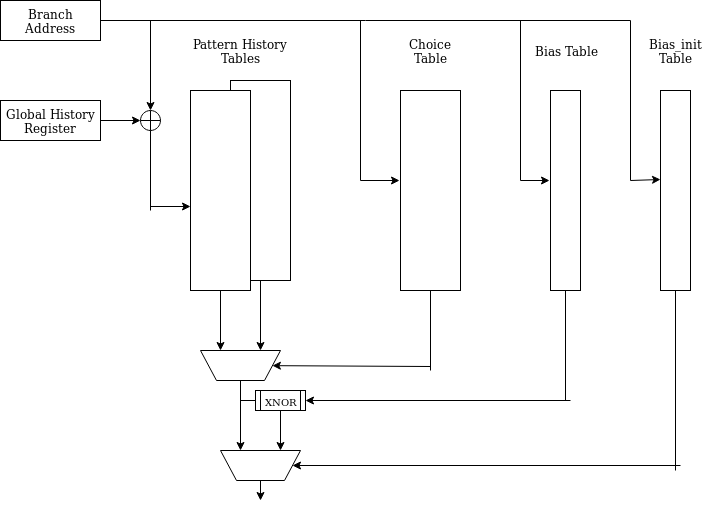
\includegraphics[scale=0.35]{agree-bimode.png}
    \caption{Block diagram for the proposed predictor model}
    \label{fig:fig1}
\end{figure}

\section{Hardware Budget}

The available budget of 64 Kbits has to be divided into 4 tables, 2 Pattern History Table, 1 Choice Table and 1 Bias table. The first three tables(2 PHTs and CPT), use 2-bit counters which the bias table stores only booleans. The implementation of bias table requires another set of counters. These counters denote if their corresponding counter in the bias table has been initialized yet. These table will furthered be referred by bias\_init table. \par

The budget is distributed among the above table as follows:
\begin{enumerate}
    \item PHT: Two table of 2-bit counters with $2^{13}$ counters each. i.e. total $2^{15}$ bits
    \item Choice table: One table with 2-bit counters with $2^{13}$ counters. i.e. total $2^{14}$ bits
    \item Bias table: $2^{13}$ one bit counters. i.e. $2^{13}$ bits
    \item Bias\_init table: similar to Bias table with $2^{13}$ bit counters.
\end{enumerate}

The above sum upto $2^{16}$ bits, i.e. 64 Kilobits. Besides these, a global branch history register is maintained for last 13 branches. which uses a 13 bit counter to store the history. This leads to a total hardware budget of $64K + 13$ bits\par

\subsection{Results and Analysis}

The following table tabulates the results obtained for our combined bimode predictor, compared to the individual components and gshare.

\begin{table}[h]

\caption{Agree\cite{agreepaper}, Bimode\cite{bimodepaper} and Gshare\cite{gsharepaper}}
\centering
\begin{tabular}{lllll}
\hline
Trace & Agree & Bimode & Gshare & Combined \\
\hline
DIST-INT-1 & 8.265 & 8.023 & 7.907 & 7.852 \\
DIST-INT-2 & 9.206 & 8.844 & 8.708 & 8.869 \\
DIST-INT-3 & 13.184 & 13.854 & 13.357 & 13.182 \\
DIST-MM-1 & 9.164 & 9.230 & 9.119 & 9.466 \\
DIST-MM-2 & 10.730 & 10.884 & 10.854 & 10.810 \\
DIST-SERV-1 & 5.319 & 3.660 & 5.691 & 4.128 \\
DIST-SERV-2 & 5.031 & 3.711 & 5.897 & 4.091 \\
DIST-SERV-3 & 5.999 & 5.698 & 7.235 & 6.185 \\
DIST-SERV-4 & 6.574 & 4.720 & 7.009 & 5.435 \\
DIST-SERV-5 & 5.431 & 4.541 & 6.767 & 4.769 \\
\hline
\end{tabular}
\end{table}

The average values overall the traces are as follows
\begin{table}[h]

\caption{Agree\cite{agreepaper}, Bimode\cite{bimodepaper} and Gshare\cite{gsharepaper}}
\centering
\begin{tabular}{llll}
\hline
Agree & Bimode & Gshare & Combined \\
\hline
7.8903 & 7.3165 & 8.254 & 7.478 \\
\hline
\end{tabular}
\end{table}

The observation we draw from the results is that our combined predictor clearly does not perform as good as the bimode predictor. This is may be because we have decreased the size of the choice predictor table to accommodate the bias bits for the agree predictions. We also observe that our predictor performs better on certain traces where the bimode does not perform as well but agree does. We observe that out combined predictor beats gshare on more traces than bimode, which implies that our predictor is somewhat more general and can be used in various traces, whereas the the bimode performs very well on only a few of them.

%%%%%%% -- PAPER CONTENT ENDS -- %%%%%%%%

%%%%%%%%% -- BIB STYLE AND FILE -- %%%%%%%%
\bibliographystyle{ieeetr}
\bibliography{ref}
%%%%%%%%%%%%%%%%%%%%%%%%%%%%%%%%%%%%

\end{document}
